% Copyright 2004 by Till Tantau <tantau@users.sourceforge.net>.
%
% In principle, this file can be redistributed and/or modified under
% the terms of the GNU Public License, version 2.
%
% However, this file is supposed to be a template to be modified
% for your own needs. For this reason, if you use this file as a
% template and not specifically distribute it as part of a another
% package/program, I grant the extra permission to freely copy and
% modify this file as you see fit and even to delete this copyright
% notice. 

\documentclass{beamer}
\usepackage[utf8]{inputenc}
\usepackage{amsmath}
\usepackage{amssymb}
\usepackage{algorithmic}
\usepackage{algorithm}
\usepackage{wrapfig}
\usepackage{longtable}
\usepackage{graphicx}
\usepackage{color}
\usepackage{listings}

\definecolor{dkgreen}{rgb}{0,0.6,0}
\definecolor{gray}{rgb}{0.5,0.5,0.5}
\definecolor{black}{rgb}{0,0,0}
\definecolor{blue}{rgb}{0,0,0.4}
\definecolor{purple}{rgb}{0.8,0,0.3}
\definecolor{orange}{rgb}{1,0.4,0}

\newcommand{\codec}[1]{
\footnotesize
  \mbox{
    \lstset{framexleftmargin=5mm, frame=shadowbox, rulesepcolor=\color{gray}}
    \lstinputlisting[language=C,
      breaklines=true,
      basicstyle=\footnotesize\ttfamily,
      keywordstyle=\bfseries\color{dkgreen},
      commentstyle=\itshape\color{purple},
      identifierstyle=\color{blue},
      stringstyle=\color{orange},
      showstringspaces=false]{#1}
  }
}

% There are many different themes available for Beamer. A comprehensive
% list with examples is given here:
% http://deic.uab.es/~iblanes/beamer_gallery/index_by_theme.html
% You can uncomment the themes below if you would like to use a different
% one:
%\usetheme{AnnArbor}
%\usetheme{Antibes}
%\usetheme{Bergen}
%\usetheme{Berkeley}
%\usetheme{Berlin}
%\usetheme{Boadilla}
%\usetheme{boxes}
%\usetheme{CambridgeUS}
%\usetheme{Copenhagen}
%\usetheme{Darmstadt}
%\usetheme{default}
%\usetheme{Frankfurt}
%\usetheme{Goettingen}
%\usetheme{Hannover}
%\usetheme{Ilmenau}
%\usetheme{JuanLesPins}
%\usetheme{Luebeck}
\usetheme{Madrid}
%\usetheme{Malmoe}
%\usetheme{Marburg}
%\usetheme{Montpellier}
%\usetheme{PaloAlto}
%\usetheme{Pittsburgh}
%\usetheme{Rochester}
%\usetheme{Singapore}
%\usetheme{Szeged}
%\usetheme{Warsaw}

\title{Implementação Paralela para GPU de uma Máquina de Vetores Suporte Usando o Algoritmo Kernel-Adatron}

% A subtitle is optional and this may be deleted
%\subtitle{Optional Subtitle}

\author{Felipe Sepulveda de Faria}
% - Give the names in the same order as the appear in the paper.
% - Use the \inst{?} command only if the authors have different
%   affiliation.

\institute[Universidade Federal do Rio de Janeiro]
{
  Departamento de Ciência da Computação\\
  Universidade Federal do Rio de Janeiro
}
% - Use the \inst command only if there are several affiliations.
% - Keep it simple, no one is interested in your street address.

\date{Projeto Final de Curso, Junho de 2016}
% - Either use conference name or its abbreviation.
% - Not really informative to the audience, more for people (including
%   yourself) who are reading the slides online

%\subject{Theoretical Computer Science}
% This is only inserted into the PDF information catalog. Can be left
% out. 

% If you have a file called "university-logo-filename.xxx", where xxx
% is a graphic format that can be processed by latex or pdflatex,
% resp., then you can add a logo as follows:

\pgfdeclareimage[height=0.5cm]{university-logo}{university-logo-filename}
\logo{\pgfuseimage{university-logo}}

% Delete this, if you do not want the table of contents to pop up at
% the beginning of each subsection:
%\AtBeginSubsection[]
%{
%  \begin{frame}<beamer>{Outline}
%    \tableofcontents[currentsection,currentsubsection]
%  \end{frame}
%}

% Let's get started
\begin{document}

\begin{frame}
  \titlepage
\end{frame}

\begin{frame}{Outline}
  \tableofcontents
  % You might wish to add the option [pausesections]
\end{frame}

% Section and subsections will appear in the presentation overview
% and table of contents.
\section{Introdução}

\subsection{MVS - Máquina de Vetores Suporte}

\begin{frame}{MVS}{Máquina de Vetores Suporte}
  \begin{itemize}
  \item {
    Aprendizado de Máquina
  }
  \item {
    Algoritmo Kernel-Adatron
  }
  \end{itemize}
\end{frame}

\subsection{Paralelização em GPU}

\begin{frame}{Paralelização em GPU}
  \begin{itemize}
  \item {
    Alto grau de paralelismo
  }
  \item {   
    Tradicionalmente usados para Computação Gráfica
  }
  \item {
    Usados para aplicações gerais com CUDA, OpenCL e outros
  }
  \end{itemize}
\end{frame}

\subsection{Estudos}

\begin{frame}{Estudos}
  \begin{itemize}
  \item {
    Chang e Lin 2011, LIBSVM: A library for support vector machines
  }
  \item {   
    Catanzaro, Sundaram e Keutzer 2008, Fast support vector machine training and classification on graphics processors
  }
  \item {
    Carpenter 2009, Cusvm: A CUDA implementation of support vector classification and regression
  }
  \item {
    Athanasopoulos, Dimou, Mezaris, Kompatsiaris 2011, GPU acceleration for support vector machines
  }
  \end{itemize}
\end{frame}

\subsection{Objetivo}

\begin{frame}{Objetivo}
  \begin{itemize}
  \item {
    Implementar uma versão sequencial e paralela
  }
  \item {   
    Usar o algoritmo Kernel-Adatron pois é simples de entender e altamente paralelizável
  }
  \end{itemize}
\end{frame}

\subsection{Métricas de avaliação}

\begin{frame}{Métricas de avaliação}
  \begin{itemize}
  \item {
    Classificação: porcentagem de acertos
  }
  \item {   
    Paralelização: ganho de velocidade na versão paralela
  }
  \end{itemize}
\end{frame}

\section{Máquina de Vetores Suporte}

\begin{frame}{Máquina de Vetores Suporte}
  \begin{itemize}
  \item {
    Uma classe de algoritmos de aprendizado de máquina
  }
  \item {
    Essencialmente um classificador binário 
  }
  \item {
    Pode ser modificado para regressão ou multi classificação
  }
  \item {
    Usado em reconhecimento de escrita, bioinformática, mineração de dados e outros
  }
  \item {
    Iniciamos com um classificador binário, já que os outros métodos são expansões do modelo básico
  }
  \end{itemize}
\end{frame}

\begin{frame}{Superfícies de Decisão Lineares}
\begin{columns}
    \begin{column}{.49\textwidth}
    \begin{figure}
      \centering
      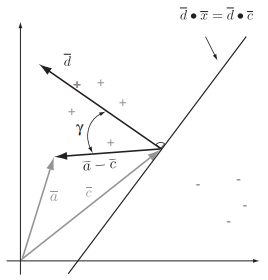
\includegraphics[width=0.8\textwidth]{svm_1.png}
    \end{figure}
    \end{column}
    \begin{column}{.49\textwidth}
      \begin{itemize}
      \item {
        Um classificador simples
      }
      \item {
        Exemplos são representados como pontos no espaço e uma superfície separa os exemplos de cada classe
      }
      \item {
        O conjunto de dados tem que ser linearmente separável
      }
      \end{itemize}
    \end{column}
\end{columns}
\end{frame}

\begin{frame}{Perceptron}
\begin{columns}
    \begin{column}{.49\textwidth}
    Essa superfície pode ser encontrada usando um perceptron
      \begin{enumerate}
      \item {
        Um classificador simples
      }
      \item {
        Exemplos são representados como pontos no espaço e uma superfície separa os exemplos de cada classe
      }
      \item {
        O conjunto de dados tem que ser linearmente separável
      }
      \end{enumerate}
    \end{column}
    \begin{column}{.49\textwidth}
    \begin{figure}
      \centering
      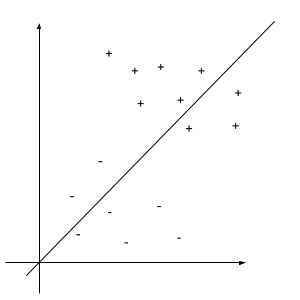
\includegraphics[width=0.8\textwidth]{perceptron_1.png}
    \end{figure}
    \end{column}
\end{columns}
\end{frame}

\begin{frame}{Perceptron}
\begin{columns}
    \begin{column}{.49\textwidth}
    Essa superfície pode ser encontrada usando um perceptron
      \begin{enumerate}
      \item {
        Um classificador simples
      }
      \item {
        Exemplos são representados como pontos no espaço e uma superfície separa os exemplos de cada classe
      }
      \item {
        O conjunto de dados tem que ser linearmente separável
      }
      \end{enumerate}
    \end{column}
    \begin{column}{.49\textwidth}
    \begin{figure}
      \centering
      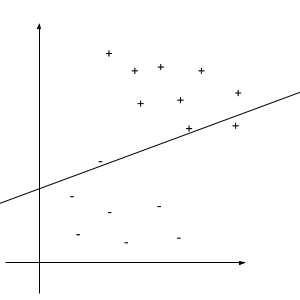
\includegraphics[width=0.8\textwidth]{perceptron_2.png}
    \end{figure}
    \end{column}
\end{columns}
\end{frame}

\begin{frame}{Perceptron}
\begin{columns}
    \begin{column}{.49\textwidth}
    Essa superfície pode ser encontrada usando um perceptron
      \begin{enumerate}
      \item {
        Um classificador simples
      }
      \item {
        Exemplos são representados como pontos no espaço e uma superfície separa os exemplos de cada classe
      }
      \item {
        O conjunto de dados tem que ser linearmente separável
      }
      \end{enumerate}
    \end{column}
    \begin{column}{.49\textwidth}
    \begin{figure}
      \centering
      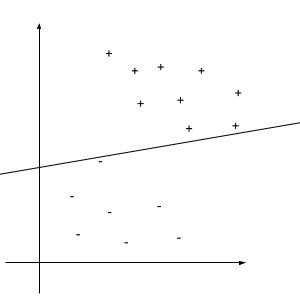
\includegraphics[width=0.8\textwidth]{perceptron_3.png}
    \end{figure}
    \end{column}
\end{columns}
\end{frame}

\begin{frame}{Margem Máxima}
\begin{columns}
    \begin{column}{.49\textwidth}
      \begin{itemize}
      \item {
        O perceptron encontra alguma superfície de separação
      }
      \item {
        Não necessariamente a melhor
      }
      \item {
        Pontos $-^*$ e $+^*$ seriam classificados errados
      }
      \item A nova superfície classifica corretamente todos os pontos
      \end{itemize}
    \end{column}
    \begin{column}{.49\textwidth}
    \begin{figure}
      \centering
      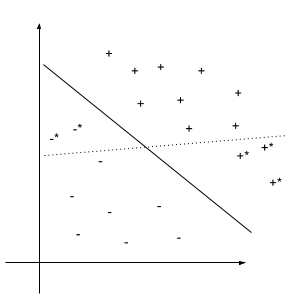
\includegraphics[width=0.8\textwidth]{margem_1.png}
    \end{figure}
    \end{column}
\end{columns}
\end{frame}

\begin{frame}{Margem Máxima}
\begin{columns}
    \begin{column}{.49\textwidth}
      \begin{itemize}
      \item Para conseguir a reta que melhor divide o espaço devemos maximizar a margem que divide as classes no espaço
      \item Hiperplanos suporte definem a fronteira da margem
      \item Vetores suporte são os exemplos que pertencem ao hiperplano de suporte
      \end{itemize}
    \end{column}
    \begin{column}{.49\textwidth}
    \begin{figure}
      \centering
      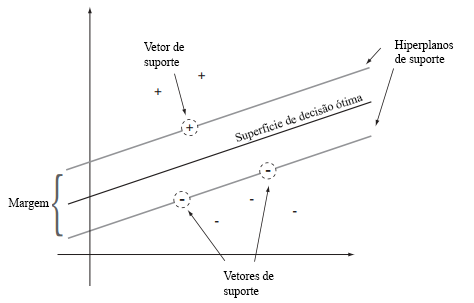
\includegraphics[width=0.9\textwidth]{svm_3.png}
    \end{figure}
    \end{column}
\end{columns}
\end{frame}

\begin{frame}{Margem Máxima}
\begin{columns}
    \begin{column}{.49\textwidth}
        \begin{equation}
        \begin{split}
        m^* &= |\bar{x}_p-\bar{x}_q|cos\gamma\\
            &= \frac{\bar{w}^*\cdot(\bar{x}_p-\bar{x}_q)}{|\bar{w}^*|}\\
            &= \frac{\bar{w}^*\cdot\bar{x}_p-\bar{w}^*\cdot\bar{x}_q}{|\bar{w}^*|}\\
            &= \frac{(b^*+k)-(b^*-k)}{|\bar{w}^*|}\\
            &= \frac{2k}{|\bar{w}^*|}
        \end{split}
        \end{equation}
    \end{column}
    \begin{column}{.49\textwidth}
    \begin{figure}
      \centering
      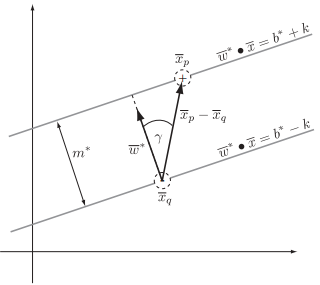
\includegraphics[width=0.9\textwidth]{svm_4.png}
    \end{figure}
    \end{column}
\end{columns}
\end{frame}

\begin{frame}{Margem Máxima}
\begin{columns}
    \begin{column}{.49\textwidth}
        \begin{equation}
        \begin{split}
        m^*=\frac{2k}{|\bar{w}^*|} &= max \frac{2k}{|\bar{w}|} \\
            &= min \frac{|\bar{w}|}{2k} \\
            &= min \frac{|\bar{w}|^2}{2k}  \\
            &= min \frac{1}{2k} \bar{w}\cdot\bar{w}  \\
            &= min \frac{1}{2} \bar{w}\cdot\bar{w}
        \end{split}
        \end{equation}
    \end{column}
    \begin{column}{.49\textwidth}
    \begin{figure}
      \centering
      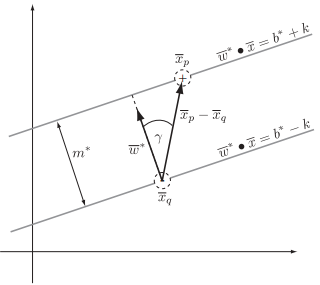
\includegraphics[width=0.9\textwidth]{svm_4.png}
    \end{figure}
    \end{column}
\end{columns}
\end{frame}

\begin{frame}{Margem Máxima}
\begin{columns}
    \begin{column}{.59\textwidth}
        \begin{equation}
            \begin{split}
                \bar{w}^*\cdot\bar{x}_i \ge b^*+k \quad \forall (\bar{x}_i,y_i)\in D \quad | \quad y_i=+1 \\
                \bar{w}^*\cdot\bar{x}_i \le b^*-k \quad \forall (\bar{x}_i,y_i)\in D \quad | \quad y_i=-1 \\
                \bar{w}^*\cdot\bar{x}_i \ge 1+b \quad \forall (\bar{x}_i,y_i)\in D \quad | \quad y_i=+1 \\
                \bar{w}^*\cdot(-\bar{x}_i) \ge 1-b \quad \forall (\bar{x}_i,y_i)\in D \quad | \quad y_i=-1
            \end{split}
        \end{equation}
    \end{column}
    \begin{column}{.39\textwidth}
    \begin{figure}
      \centering
      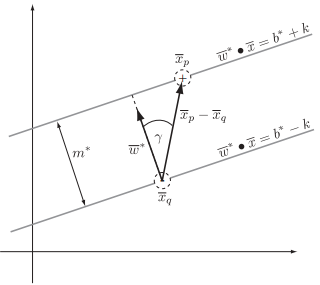
\includegraphics[width=0.9\textwidth]{svm_4.png}
    \end{figure}
    \end{column}
\end{columns}
\centering
$\bar{w}^*\cdot(y_i\bar{x}_i) \ge 1+y_i b \quad \forall (\bar{x}_i,y_i)\in D$
\end{frame}

\begin{frame}{Classificador de Margem Máxima}
\begin{itemize}
    \item Dado um conjunto de dados linearmente separáveis $D=(\bar{x}_i,y_i) \subseteq \mathbb{R}^n\times\{+1,1\}$, podemos encontrar a superfície máxima de separação, $\bar{w}^*\cdot\bar{x}=b^*$, otimizando o problema $min\phi(\bar{w},b) = \underset{\bar{w},b}{min}\frac{1}{2}\bar{w}\cdot\bar{w}$.
    \item Sujeito às restrições da Equação: $\bar{w}^*\cdot(y_i\bar{x}_i) \ge 1+y_i b \quad \forall (\bar{x}_i,y_i)\in D$.
\end{itemize}
\end{frame}

\begin{frame}{Dual Lagrangiana}
\begin{itemize}
    \item A dual lagrangiana reescreve um problema do formato: $\underset{\bar{x}}{min}\phi(\bar{x})$ dado que $h_i(\bar{x})\ge c_i$
    \item Para o formato: $\underset{\bar{\alpha}}{max} \underset{\bar{x}}{min} L(\bar{\alpha},\bar{x}) = \underset{\bar{\alpha}}{max} \underset{\bar{x}}{min}\bigg(\phi(\bar{x})-\sum_{i=1}^{l}\alpha_i g_i(\bar{x})\bigg)$ dado que $\alpha_i\ge0$.
    \item Onde $g_i(\bar{x})=h_i(\bar{x})-c_i$
\end{itemize}
\end{frame}

\begin{frame}{Dual Lagrangiana}
\begin{itemize}
    \item Encontrados os valores máximo de $\alpha^*$ e mínimo de $x^*$ a solução do problema dual será a mesma do problema primal, contanto que as seguintes condições se apliquem:
\end{itemize}
\begin{equation}
\begin{split}
\frac{\partial L}{\partial \bar{x}}(\bar{\alpha}^*,\bar{x})&=\bar{0}, \\
\alpha_i^*g_i(\bar{x}^*)&=\bar{0}, \\
g_i(\bar{x}^*)&\ge\bar{0} , \\
\bar{\alpha}_i^*(\bar{x}^*)&\ge\bar{0} 
\end{split}
\end{equation}
\begin{itemize}
    \item Essas condições são conhecidas como as condições de Karush-Kuhn-Tucker ou KKT, e podemos usá-las para reescrever nosso problema dependendo somente de $\bar{\alpha}$, facilitando nossa busca.
\end{itemize}
\end{frame}

\begin{frame}{Dual Lagrangiana}
    \begin{itemize}
        \item Agora podemos aplicar essa técnica ao nosso problema de margem máxima, escrevendo nossa função lagrangiana como:
    \end{itemize}
    \begin{equation}
        \begin{split}
            L(\bar{\alpha},\bar{w},b) &=\phi(\bar{w},b) -  \sum_{i=1}^{l}\alpha_i g_i (\bar{w},b) \\
             &=\frac{1}{2}\bar{w}\cdot\bar{w} - \sum_{i=1}^{l}\alpha_i (y_i(\bar{w}\cdot \bar{x}_i -b)-1) \\
             &=\frac{1}{2}\bar{w}\cdot\bar{w} - \sum_{i=1}^{l}\alpha_i y_i \bar{w}\cdot \bar{x}_i + b \sum_{i=1}^{l}\alpha_i y_i + \sum_{i=1}^{l}\alpha_i\\
        \end{split}
    \end{equation}
\end{frame}

\begin{frame}{Dual Lagrangiana}
Aplicando as KKTs chegamos ao nosso treinador de margem máxima dual:
\begin{equation}
    \underset{\bar{\alpha}}{max} \phi' (\bar{\alpha}) = \underset{\bar{\alpha}}{max} \Bigg( \sum_{i=1}^{l}\alpha_i - \frac{1}{2}\sum_{i=1}^{l}\sum_{j=1}^{l}\alpha_i \alpha_j y_i y_j \bar{x}_i\cdot \bar{x}_j \Bigg)
\end{equation}
dado que:
\begin{equation}
    \sum_{i=1}^{l}\alpha_i y_i = 0 \quad \text{e} \quad \alpha_i \ge 0 \quad \forall  i \in \{1,l\}
\end{equation}
\end{frame}

\begin{frame}{Dual Lagrangiana}
Uma vez encontrado nosso $\bar{\alpha}^*$ ótimo, podemos classificar um novo ponto $\bar{x}$ com a fórmula:
\begin{equation}
    f(\bar{x}) = sgn\Bigg(
        \sum_{i=1}^{l} \alpha_i^*y_i\bar{x}_i\cdot\bar{x}
        -b^*
    \Bigg)
\end{equation}

\begin{equation}
    b^* = \sum_{i=1}^{l} 
    \Bigg(
        \alpha_i^*y_i\bar{x}_i\cdot\bar{x}_{sv+} -1
    \Bigg)
\end{equation}
\end{frame}

\begin{frame}{Truque do Kernel}
\begin{itemize}
    \item O truque do kernel é usado para poder classificar conjuntos de dados que não sejam linearmente separáveis
    \item Escolhemos funções de projeção que aumentem a dimensão do conjunto de dados na esperança de que nesse espaço eles possam ser linearmente separáveis
\end{itemize}
\end{frame}

\begin{frame}{Truque do Kernel}
\begin{figure}
    \centering
    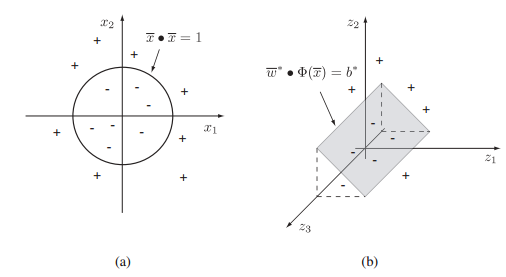
\includegraphics[width=0.9\textwidth]{svm_5.png}
\end{figure}
\end{frame}

\begin{frame}{Truque do Kernel}
\begin{itemize}
    \item como sempre usamos o produto de $\phi$ podemos simplificar seu resultado
\end{itemize}
        \begin{equation}
        \begin{split}
        \phi(\bar{x})\cdot \phi(\bar{y}) &= (x_1^2,x_2^2,\sqrt{2}x_1x_2) \cdot (y_1^2,y_2^2,\sqrt{2}y_1y_2) \\
        &=x_1^2y_1^2+x_2^2y_2^2+2x_1x_2y_1y_2 \\
        &=(x_1y_1+x_2y_2)(x_1y_1+x_2y_2) \\
        &=(\bar{x}\cdot\bar{y})(\bar{x}\cdot\bar{y}) \\
        &=(\bar{x}\cdot\bar{y})^2
        \end{split}
        \end{equation}
\end{frame}

\begin{frame}{Truque do Kernel}
\begin{table}
    \small
    \centering
    \begin{tabular}{|c|c|c|} \hline
            Kernel & Função & Parâmetros Livres \\ \hline
        Kernel Linear & $k(\bar{x},\bar{y})=\bar{x}\cdot\bar{y}$ & nenhum \\
        Kernel Homogêneo Polinomial & $k(\bar{x},\bar{y})=(\bar{x}\cdot\bar{y})^d$ & $d\ge2$ \\
        Kernel Não-Homogêneo Polinomial & $k(\bar{x},\bar{y})=(\bar{x}\cdot\bar{y}+c)^d$ & $d\ge2, c > 0$ \\
        Kernel Gaussiano & $k(\bar{x},\bar{y})=e^{-\big(\frac{|\bar{x}-\bar{y}|^2}{2\sigma^2}\big)}$ & $\sigma>0$ \\ \hline
    \end{tabular}
\end{table}
\end{frame}

\begin{frame}{MVS com Truque do Kernel}
Treinador:
\begin{equation}
    \bar{\alpha}^* = \underset{\bar{\alpha}}{argmax}{\phi}'(\bar{\alpha}) =\underset{\bar{\alpha}}{argmax} \Bigg( \sum_{i=1}^{l}\alpha_i - \frac{1}{2}\sum_{i=1}^{l}\sum_{j=1}^{l}\alpha_i \alpha_j y_i y_j k(\bar{x}_i,\bar{x}_j) \Bigg)
    \label{eq:EQ_Treinador_2}
\end{equation}
Classificador:
\begin{equation}
    f(\bar{x}) = sgn\Bigg(
        \sum_{i=1}^{l} \alpha_i^*y_i k(\bar{x}_i,\bar{x})
        -b^*
    \Bigg)
    \label{eq:EQ_Classificador_2}
\end{equation}
\begin{equation}
    b^* = \sum_{i=1}^{l}
    \Bigg(
        \alpha_i^*y_i k(\bar{x}_i,\bar{x}_{sv+})-1
    \Bigg)
    \label{eq:EQ_B_2}
\end{equation}
\end{frame}

\begin{frame}{Margem Flexível}
\begin{figure}
    \centering
    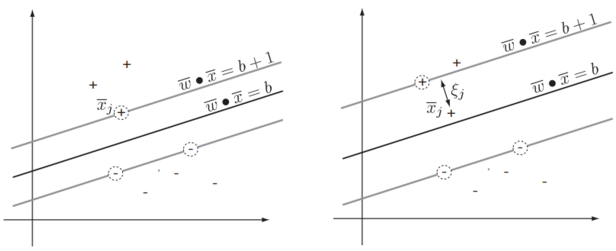
\includegraphics[width=0.9\textwidth]{svm_6.png}
\end{figure}
$\underset{\bar{w}, \bar{\epsilon}, b}{min}\phi(\bar{w}, \bar{\epsilon},b)
    = \underset{\bar{w}, \bar{\epsilon}, b}{min}\frac{1}{2}\bar{w}\cdot\bar{w} + C\sum_{i=1}^l \epsilon_i
    = \frac{1}{2}\bar{w}^*\cdot\bar{w}^* + C\sum_{i=1}^l \epsilon_i^*
    =m^*$
\end{frame}

\begin{frame}{Gradiente Ascendente}
\begin{columns}
\begin{column}{0.49\textwidth}
    \begin{itemize}
        \item Utiliza o gradiente de $\alpha$ como incremento para chegar no ponto ótimo
        \item $\triangledown_i {\phi}'(\bar{\alpha}) = 1-y_i\sum_{j=1}^ly_j\alpha_jk(\bar{x}_j,\bar{x}_i)$
    \end{itemize}
\end{column}
\begin{column}{0.49\textwidth}
\begin{enumerate}
    \item $\eta>0$
    \item $\bar{\alpha} \leftarrow \bar{0}$
    \item repeat
    \item $\quad$ $\bar{\alpha_{old}} \leftarrow \bar{\alpha}$
    \item $\quad$ for $i=1$ to $l$
    \item $\quad$ $\quad$ $\quad$ $\alpha_i \leftarrow a_i + \eta \triangledown_i {\phi}'(\bar{\alpha})$
    \item $\quad$ end for
    \item until $\bar{\alpha}-\bar{\alpha_{old}}\approx \bar{0}$
    \item return $\bar{\alpha}$
\end{enumerate}
\end{column}
\end{columns}
\end{frame}

\begin{frame}{Kernel-Adatron}
\begin{columns}
\begin{column}{0.39\textwidth}
    \begin{itemize}
        \item Possui margem flexível
        \item Fixa o valor de $b$
        \item Possui as restrições: $\alpha_i \ge 0$ e $\alpha_i \le C$
    \end{itemize}
\end{column}
\begin{column}{0.59\textwidth}
\begin{enumerate}
    \item $D = \{(\bar{x_i},y_1)...(\bar{x_i},y_1)\} \subset \mathbb{R}^{n}\times \{+1,-1\}$
    \item $\eta>0$
    \item $C>0$
    \item $b=0$
    \item $\bar{\alpha} \leftarrow \bar{0}$
    \item repeat
    \item $\bar{\alpha_{old}} \leftarrow \bar{\alpha}$
    \item for$i=1$ to $l$
    \item $\alpha_i \leftarrow min\big\{C,max\big\{0,\alpha_i + \eta-\eta y_i \sum_{j=1}^l y_j \alpha_j k(\bar{x}_j,\bar{x}_i))\big\}\big\}$
    \item end for
    \item until $\bar{\alpha}-\bar{\alpha_{old}}\approx \bar{0}$
    \item return $(\bar{\alpha},b)$
\end{enumerate}
\end{column}
\end{columns}
\end{frame}

\begin{frame}{Quadratic Program Solver}
\begin{itemize}
    \item Algoritmo de otimização que encontra os valores de um parâmetro que minimizam uma função dado um conjunto de restrições
    \item Várias bibliotecas implementam esse algoritmo
\end{itemize}
\end{frame}

\begin{frame}{SMO: Sequential Minimal Optimization}
\begin{itemize}
    \item Otimiza dois pontos de cada vez até que as restrições de KKT não sejam violadas
    \item Os pontos são escolhidos de forma que um respeite as restrições e o outro seja o maior violador
    \item O algoritmo sempre converge
    \item Isso permite uma série de otimizações em cima das fórmulas vistas
\end{itemize}
\end{frame}

\section{Programação Paralela}

\begin{frame}{Programação Paralela}
Distribuir o processamento de um programa com a finalidade de reduzir o tempo total de execução.

Os programas podem executar:
\begin{itemize}
    \item Em diferentes núcleos de um mesmo computador, dividindo o processamento em diferentes threads ou processos
    \item Em diferentes máquinas, através de um cluster ou computação em nuvem
    \item Em uma CPU auxiliada por dispositivos aceleradores, como por exemplo, uma GPU
\end{itemize}
\end{frame}

\begin{frame}{GPUs - Graphics Processing Units}
Originalmente projetadas como aceleradores gráficos.

Aplicações:
\begin{itemize}
    \item Alterar a cor de todos os pixels de uma imagem
    \item Rotacionar e transladar polígonos com muitos pontos
    \item Aplicar texturas em polígonos
    \item Calcular luminosidade em polígonos
\end{itemize}
Muitas operações são feitas em pontos distintos de forma independente.
\end{frame}

\begin{frame}{GPUs X CPUs}
\begin{columns}
\begin{column}{0.44\textwidth}
\begin{itemize}
    \item Possuem de centenas a milhares de unidades lógicas
    \item Menos espaço dedicado ao controle de fluxo e cache
    \item Maior paralelismo
\end{itemize}
\end{column}
\begin{column}{0.54\textwidth}
\begin{figure}
    \centering
    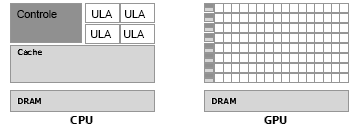
\includegraphics[width=1\textwidth]{gpu_1.png}
\end{figure}
\end{column}
\end{columns}
\end{frame}

\begin{frame}{CUDA}
\begin{itemize}
    \item Lançado em 2006
    \item Plataforma de computação e modelo de programação.
    \item Permite que desenvolvedores explorem o potencial das GPUs para aplicações de propósito geral.
    \item É possível usar C, C++ e Fortran
\end{itemize}
\end{frame}

\begin{frame}{CUDA}
\begin{itemize}
    \item As threads são organizadas em blocos.
    \item Threads de um mesmo bloco são executados no mesmo núcleo e compartilham uma área de memória.
    \item Dentro de um bloco as threads são agrupadas em warps (conjunto de 32 threads).
    \item Os warps são as unidades de escalonamento para execução: todas as threads do warp executam ao mesmo tempo a mesma instrução.
    %\item Cada warp executa perfeitamente em paralelo.
\end{itemize}
\end{frame}

\begin{frame}{CUDA}
    \codec{codigos/cuda_1.txt}
\end{frame}

\begin{frame}{CUDA}
    \codec{codigos/cuda_2.txt}
\end{frame}

\section{Implementação}

\begin{frame}{Implementação}
  \begin{itemize}
    \item Kernel-Adatron: Mais custoso, maior ganho na paralelização
    \item Gradiente Ascendente: incompleto comparado ao Kernel-Adatron
    \item Quadratic Program Solver: Algoritmo genérico de otimização
    \item Sequential Minimal Optimization: Otimizado para a versão sequencial, mais complicado de paralelizar, complexo.
  \end{itemize}
\end{frame}

\begin{frame}{Comandos}
\begin{table}
\scalebox{0.9}{
    \footnotesize
    \centering
    \tabcolsep=0.11cm
    \begin{tabular}{|c|c|c|c|} \hline
        Comando & Descrição & Valores aceitos & Default \\ \hline
        -c & Constante de margem flexível & double & 999.0 \\ \hline
        -d & Conjunto de Dados &  i:Iris & i \\ 
         &  &  a[1-9]:Adult &  \\ 
         &  &  w[1-8]:Web &  \\ \hline
        -f & Partições na validação cruzada & int & 10 \\ \hline
        -g & $\gamma$ usado pelo kernel gaussiano & double & 0.5 \\ \hline
        -h & Menu de ajuda & & \\ \hline
        -l & Nível de log & a:Todos , r:Resultados  & r \\
           & & e:Erros , n:Nenhum & \\ \hline
        -mi & Máximo de Iterações & int & 128 \\ \hline
        -p & Precisão da parada & double & 1e-010 \\ \hline
        -sd & Gerador de número aleatório & int & time(nullptr) \\ \hline
        -st & Paço inicial & double & 1 \\ \hline
        -sm & Modo de Step & s:Single Step & s \\
        & & m:Multi Step & \\ \hline
        -ua & Modo estocástico & f:false | t:true & f \\ \hline
        -svm & Tipo de MVS & p:Paralelo & s \\
         &  & s:Sequencial &  \\ \hline
        -t & Threads por Bloco & int & 128 \\ \hline
    \end{tabular}   
}
\end{table}
\end{frame}

\begin{frame}{Validação Cruzada}
\begin{itemize}
    \item Para se obter as métricas usadas na avaliação, é usado um método conhecido como validação cruzada.
    \item O conjunto de dados é dividido em $n$ partições.
    \item Para cada partição $i \in [1,n]$ é feito um treinamento com as outras partições $[1,n]-i$.
    \item É feita a classificação de todas as amostras na partição $i$ para comparar com o valor real da classe de $i$ e descobrir quantos casos teste foram classificados corretamente.
    \item Isso é feito para todos os conjuntos de $n$.
    \item Todas as amostras foram classificadas uma vez e participaram de $n-1$ treinamentos.
\end{itemize}
\end{frame}

\begin{frame}{Kernel Gaussiano}
  \begin{columns}
  \begin{column}{0.39\textwidth}
    \begin{itemize}
        \item Usado nos estudos
        \item Bons resultados
    \end{itemize}
  \end{column}
  \begin{column}{0.59\textwidth}
    $k(\bar{x},\bar{y}) = e^{-\big( \frac{|\bar{x}-\bar{y}|^2} {2\sigma^2}\big)}$
    
    $\frac{1}{2\sigma^2} = \gamma$
    
    $|\bar{x}| = \sqrt{\sum x_i^2}$
    
    $|\bar{x}-\bar{y}|^2 = \bigg(\sqrt{\sum (x_i-y_i)^2}\bigg)^2=\sum (x_i-y_i)^2$
    
    $e^{\big(-\gamma*\sum (x_i-y_i)^2\big)}$
  \end{column}
  \end{columns}
\end{frame}

\begin{frame}{Kernel Gaussiano}{Código}
    \codec{codigos/gausKernel.txt}
\end{frame}

\begin{frame}{Condição de Parada}
\begin{itemize}
    \item $\bar{\alpha}-\bar{\alpha_{old}}\approx \bar{0}$.
    \item Precisamos definir o quão próximo de zero é o suficiente.
    \item $|a-b|<p$ se $a\approx b$
\end{itemize}
\begin{itemize}
    \item Existem conjuntos que podem demorar muito para terminar.
    \item Limite máximo de iterações
\end{itemize}
Condição de parada: o treinamento é interrompido quando a diferença do valor de $\alpha$ entre duas iterações é menor que $p$, ou quando atingirmos o máximo de iterações definido.
\end{frame}

\begin{frame}{Tamanho dos Incrementos}
\begin{itemize}
    \item É difícil saber o tamanho certo do incremento
    \item Se for muito grande, o algoritmo pode nunca convergir e sempre ultrapassar o ponto ótimo.
    \item Se for muito pequeno o algoritmo pode demorar muito para chegar no ponto ótimo.
\end{itemize}
A solução encontrada para o problema foi adotar um $\eta$ flexível.
\begin{itemize}
    \item Começamos com um incremento grande
    \item Quando passamos do ponto ótimo, reduzimos o incremento
\end{itemize}
\end{frame}

\begin{frame}{Tamanho dos Incrementos}
Quando passamos do ponto ótimo?
\begin{itemize}
    \item Diferença média de $\bar{\alpha}$ aumentou
    \item Diferença média de $\bar{\alpha}$ mudou de sinal
\end{itemize}
\end{frame}

\begin{frame}{Atualização do Tamanho do Incremento}{Código}
    \codec{codigos/updateStep.txt}
\end{frame}

\begin{frame}{Modo de Incremento}{StepMode}
Alguns parâmetros convergem mais rápidos que outros, para isso criamos um modo de incremento.
\begin{itemize}
    \item SingleStep: um valor de incremento para todos os $\alpha_i$
    \item MultiStep: um valor de incremento para cada $\alpha_i$
\end{itemize}
\end{frame}

\begin{frame}{Modo Estocástico}
\begin{itemize}
    \item No algoritmo Kernel-Adatron os valores de $\bar{\alpha}$ são usados assim que são descobertos.
    \item Cada valor de $\alpha_i$ influencia no cálculo de todos os outros $\rightarrow$ não é paralelo.
    \item Fizemos uma versão estocástica e outra não-estocástica para comparar os resultados
\end{itemize}
\end{frame}

\begin{frame}{Otimização Não-Estocástica}
\begin{itemize}
    \item Na primeira iteração todos os valores de $\alpha$ são nulos
    \item Na segunda iteração, todos os valores de $\alpha$ serão iguais ao incremento inicial
    \item Podemos inicializar $\alpha$ com o valor do passo inicial
\end{itemize}
\end{frame}

\begin{frame}{Treinamento Sequencial}
    \codec{codigos/SequentialSvmTrain.txt}
\end{frame}

\begin{frame}{Classificação Sequencial}
    \codec{codigos/SequentialSvmClassify.txt}
\end{frame}

\section{Implementação Paralela}

\begin{frame}{Implementação Paralela}
Desafios e gargalos:
\begin{itemize}
    \item Transferência de dados entre o host e o device
    \item Dependência de dados entre as threads
\end{itemize}
Porque o Algoritmo Kernel-Adatron é bastante paralelizável?
\begin{itemize}
    \item Vetores grandes
    \item Tarefas independentes
    \item Tarefas custosas
\end{itemize}
\end{frame}

\begin{frame}{CUDA\_SAFE\_CALL}
\codec{codigos/CUDA_SAFE_CALL.txt}
\end{frame}

\begin{frame}{CudaArray}
\codec{codigos/CudaArray.txt}
\end{frame}

\begin{frame}{initArray}
\codec{codigos/initArray.txt}
\end{frame}

\begin{frame}{Kernel-Adatron Paralelo}
Método estocástico?
\begin{itemize}
    \item A única parte paralelizável é o kernel
    \item Pouco trabalho na GPU
    \item Muita transfererência entre o host e o device
\end{itemize}
Método não-estocástico
\begin{itemize}
    \item Cada $\alpha_i$ é calculado em uma thread separada
    \item Maior parte do trabalho na GPU
    \item Somente o cálculo da condição de parada fica no host
\end{itemize}
\end{frame}


\end{document}


